% See UNHTHESIS.TEMPLATE for additional comments about this file.
%
\chapter{Background}

\section{The Model}

Both the short- and long-term effects of human exploitation on an ecosystem such as a fishery are not easily understood since experiments which would allow ecosystem managers to investigate the impact of different levels of exploitation over many years are either impractical or impossible to conduct on a large scale.  Fortunately, ecosystem models can be used instead to help gain a better understanding of an ecosystem.

Ecosystem models are abstract representations of an ecological system, which could mean anything from an individual species to an entire community of species.  A classic example is the Lotka-Volterra model, which is a pair of differential equations for describing the non-linear interactions between a predator species and a prey species. \cite{Lotka1926fds, VOL26a}:

\begin{align}
   \frac{d N_1}{dt} &=   N_1 \left(\alpha - \beta  N_2\right) 
\\ \frac{d N_2}{dt} &= - N_2 \left(\gamma - \delta N_1\right)
\end{align}
where $N_1$ is the number of prey, $N_2$ is the number of predator, $t$ is time, $\alpha$ is the prey's growth rate, $\beta$ is the rate at which the predator destroys the prey, $\gamma$ is the death rate of the predator, and $\delta$ is the rate at which the predator increases from consuming the prey.  The model can be generalized to discuss an arbitrary number of species rather than just a single pair.

The Lotka-Volterra model can be modified to take competition instead of predation into account, as in the Rosenzweig-MacArthur model \cite{Rosenzweig1963Graphical} and the Leslie-Gower model \cite{leslie1960}.  These adaptations to the model also consider carrying capacity, which is the maximum number of a species that can sustained indefinitely:

\begin{align}
   \frac{d N_1}{dt} &= r_1 N_1 \left(1 - \left(\frac{N_1 + \alpha_{12} N_2}{K_1}\right)\right)
\\ \frac{d N_2}{dt} &= r_2 N_2 \left(1 - \left(\frac{N_2 + \alpha_{21} N_1}{K_2}\right)\right)
\end{align}
where $r_i$ is the growth rate for species $i$, $K_i$ is the carrying capacity for species $i$, and $\alpha_{ij}$ is the effect species $j$ has on species $i$.  As with Lotka-Volterra, this model concerns only two species, but it can be generalized to include more than two.

Both Lotka-Volterra and Leslie-Gower do not incorporate a factor which is critical when discussing fisheries management: the effect of harvest.  The Schaefer model adds a term to account for the effect of harvest on an individual species \cite{schaefer1957}:

\begin{align}
   \frac{d N}{dt} &= r N \left(1 - \left(\frac{N}{K}\right)\right) - q E N
\end{align}
where $N$ is the number (or biomass) of the species, $r$ is the growth rate, $K$ is the carrying capacity, $q$ is the catchability coefficient, and $E$ is the fishing effort.

Simple models, when available and correct, are generally preferred; since fewer components are needed to describe their real-world counterparts, they are more easily understood and implemented.  All three of these models are subjectively simple in that they only consider a few ecological factors each. However, ecosystems are complex systems which require management that recognizes them as such \cite{Christensen1996Report}.  Thus, a more holistic approach called ecosystem-based fishery management (EBFM) has been advocated \cite{united1999ecosystem}.  However, this approach has not often been implemented due to a lack of models which consider all necessary ecological factors.  Gamble and Link developed a multispecies production model (MS-PROD) to fill this gap \cite{Gamble20092570}.

The MS-PROD model is built upon the Schaefer production model by also including Lotka-Volterra terms for predation, Leslie-Gower terms for competition, and carrying capacities for functional groups ($K_G$) as well as for the entire system ($K_{\sigma}$):

\begin{align}
\frac{d N_i}{dt} &= r_i N_i \left(1 - \frac{N_i}{K_G} - \frac{\displaystyle\sum\limits_{j=1}^g \beta_{ij} N_j}{K_G} - \frac{\displaystyle\sum\limits_{j=1}^G \beta_{ij} N_j}{K_{\sigma} - K_G}\right) - N_i \displaystyle\sum\limits_{j=1}^P \alpha_{ij} N_j - H_i N_i
\end{align}
where $N_i$ is the number (or biomass) of species $i$, $t$ is a unit of time, $r_i$ is growth rate for species $i$, $\beta_{ij}$ is the interaction of species $j$ on $i$, $\alpha_{ij}$ is the predation of species $j$ on $i$, $H_i$ is the harvest rate on species $i$, $g$ is the number of species within species $i$'s group, $G$ is the number of groups, and $p$ is the number of predators.

This model is distinguished from other multispecies production models by describing stocks with explicit ecological and harvest factors.  Ten key species were chosen from the Northeast United States Continental Shelf Large Marine Ecosystem (NEUS LME) from four major functional groups.  Given an input parameter set of initial biomass values, a predation matrix, an interaction matrix, catchability values, and harvest effort values, the MS-PROD model runs simulations for 30 years with an annual time step to predict individual biomasses.  While this outputted information is potentially valuable to fishery managers, it was lacking an interactive graphical user interface.  

\section{Visualization Methods}

\subsection{Time Series}

Fisheries management is focused on the sustainability of choices concerning fish stocks.  A main purpose of ecosystem management is to ensure future generations can enjoy the same natural resources \cite{Christensen1996Report}.  As such, the MS-PROD model provides biomass forecasts for 30 years.  Therefore, time-oriented visualization techniques must be explored.

Frank discussed the different types of time-oriented data by defining three criteria: a) linear vs. cyclic, b) time points vs. time intervals, and c) ordered time vs. branching time vs. time with multiple perspectives \cite{frank98times}.  The MS-PROD data consist of discrete time points with definite starting and ending points, falling under the linear time and time points categories.  As for the third criterion, the model outputs one ordered time result for a single execution, however fisheries managers may like to compare alternative scenarios.  Therefore, our domain falls into the branching time category.  Aigner et al. point out that techniques for visualizing branching time and time with multiple perspectives are unfortunately uncommon \cite{Aigner08visualmethods}, but a line chart---a technique frequently used for ordered time data---serves as a good starting point.

\begin{figure}[h]
	\centering
	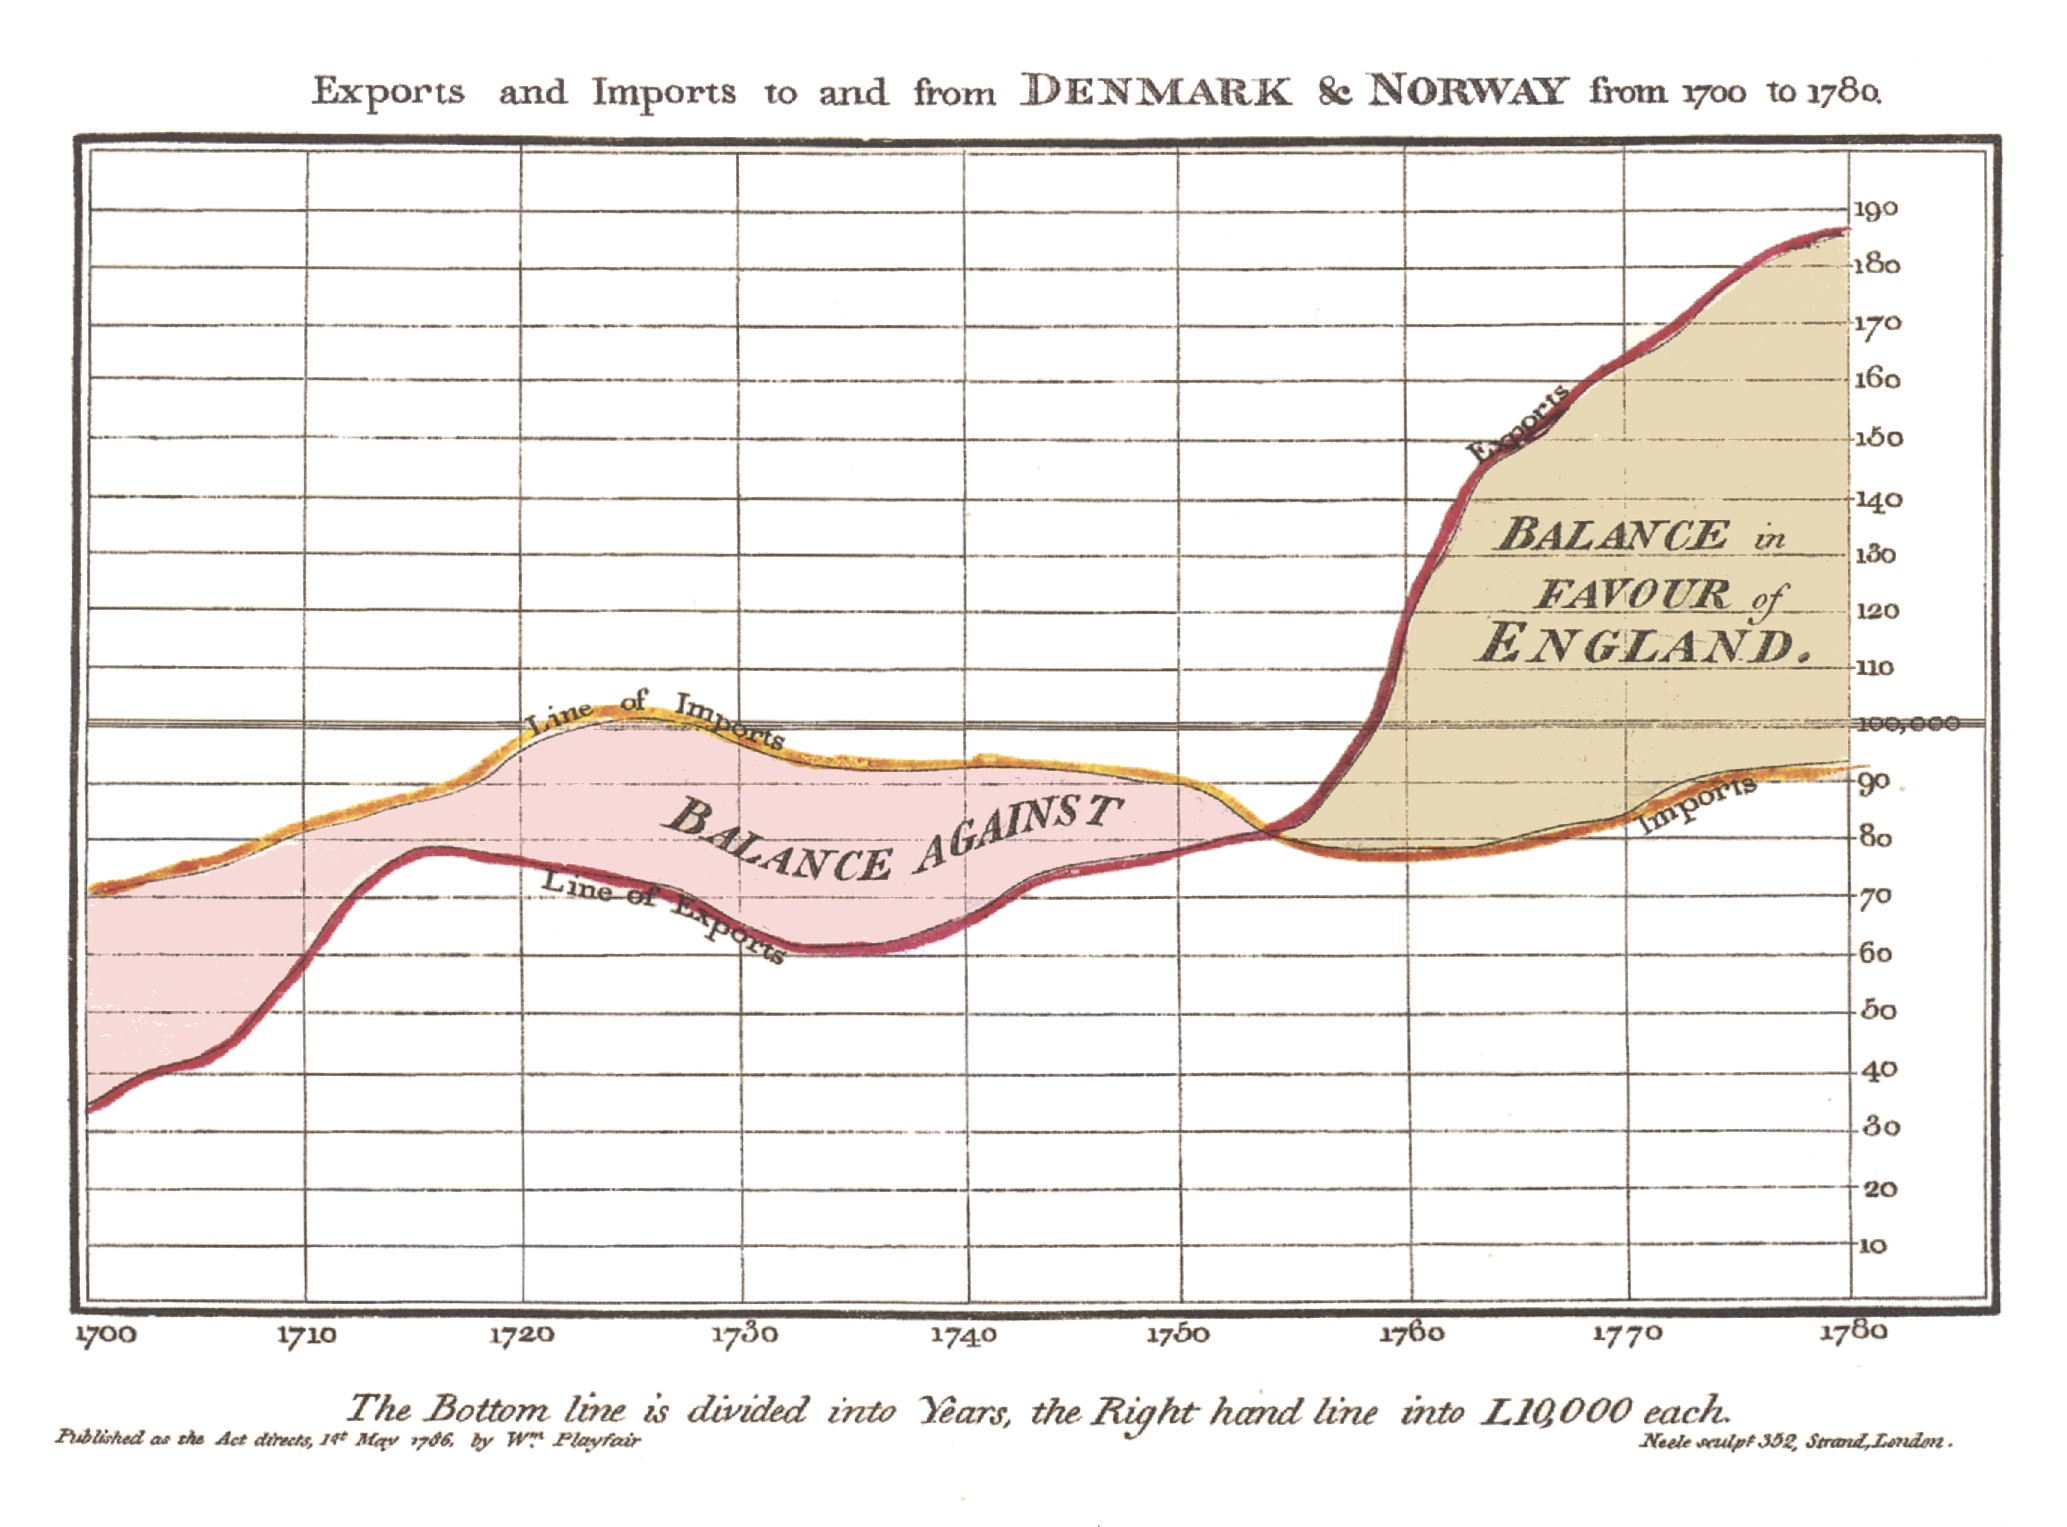
\includegraphics[width=10cm]{figures/PlayfairTimeSeries.eps}
	\caption{Playfair's original time series chart \cite{playfair}.}
	\label{fig:playfair}
\end{figure}

The line chart was first invented by William Playfair in 1786 to communicate time series data, seen in Figure~\ref{fig:playfair} \cite{playfair}.  Today, it remains a common method for visualizing time-oriented data in many fields, including science, economics, planning, and engineering to name a few.  Line charts typically encode time on the horizontal axis, progressing from left to right, and some time-varying value on the vertical axis.  Points in the chart are connected by line segments such that the slope of the line indicates the rate of change between time steps.  

\begin{figure}
	\centering
	\begin{subfigure}[b]{0.45\textwidth}
		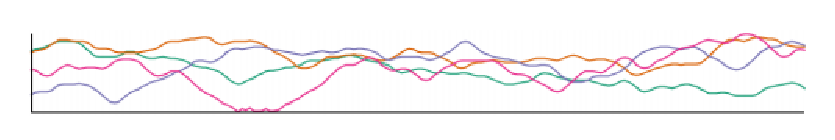
\includegraphics[width=\textwidth]{figures/ts_simplelinegraph.eps}
		\caption{A simple line graph.}
		\label{fig:ts_simple}
	\end{subfigure}
	\begin{subfigure}[b]{0.45\textwidth}
		
\includegraphics[width=\textwidth]{figures/ts_braidedgraph.eps}
		\caption{A braided graph.}
		\label{fig:ts_braid}
	\end{subfigure}
	\\
	\begin{subfigure}[b]{0.45\textwidth}
		
\includegraphics[width=\textwidth]{figures/ts_smallmultiples.eps}
		\caption{Small multiples.}
		\label{fig:ts_smmult}
	\end{subfigure}
	\begin{subfigure}[b]{0.45\textwidth}
		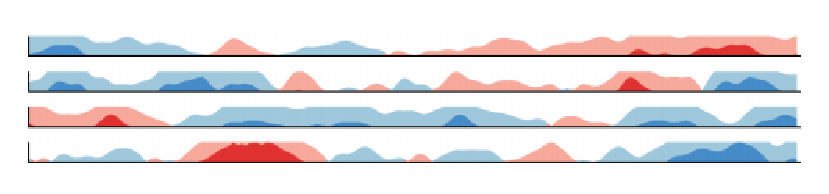
\includegraphics[width=\textwidth]{figures/ts_horizongraphs.eps}
		\caption{Horizon graphs.}
		\label{fig:ts_horizon}
	\end{subfigure}
	\caption{Four methods for visualizing multiple time series by Javed et al \cite{Javed:2010:GPM:1907651.1907971}.}
	\label{fig:ts_compare}
\end{figure}

Multiple time series can be part of a single line chart; each series needs only to be distinguished by a color and/or line style.  However, as the number of time series on a single line chart increases, it becomes more difficult to identify an individual series.  Javed et al. studied different plotting techniques for multiple time series, as seen in Figure~\ref{fig:ts_compare} \cite{Javed:2010:GPM:1907651.1907971}.  The first of their techniques is the ``simple line chart,'' which was Playfair's original line chart with all series plotted together.  A slight variation on that is ``small multiples,'' where each series had its own line chart though all charts share the same axis scales.  Horizon graphs, originally developed by Saito et al., wrap around a baseline in two color tones to save space \cite{saitoTwoTone}.  Lastly, braided graphs feature all series on one chart with the coloring under the curves alternating as series intersect each other.  The user evaluation by Javed et al. revealed that a simple line graph with all time series on one plot or a single graph for each time series is better suited to a variety of tasks than a horizon graph or a braided graph.  They also found that users complete tasks more correctly when there is more display space allocated to the graphs.  They did not recommend using a higher number of simultaneous time series---their study used eight at the most---because it also leads to a decline in correctness of task completion.

\subsection{Networks}

The input parameters to the MS-PROD model includes predation and interaction matrices.  These are relationships which may be better understood if incorporated into the visualization. Relationships are often visualized through a node-link diagram, which typically represents entities as nodes and links as relationships between the nodes they connect.  There are many types of node-link diagrams used for illustrating networks, of which only a few are discussed in the following sections.

\begin{figure}[h]
	\centering
	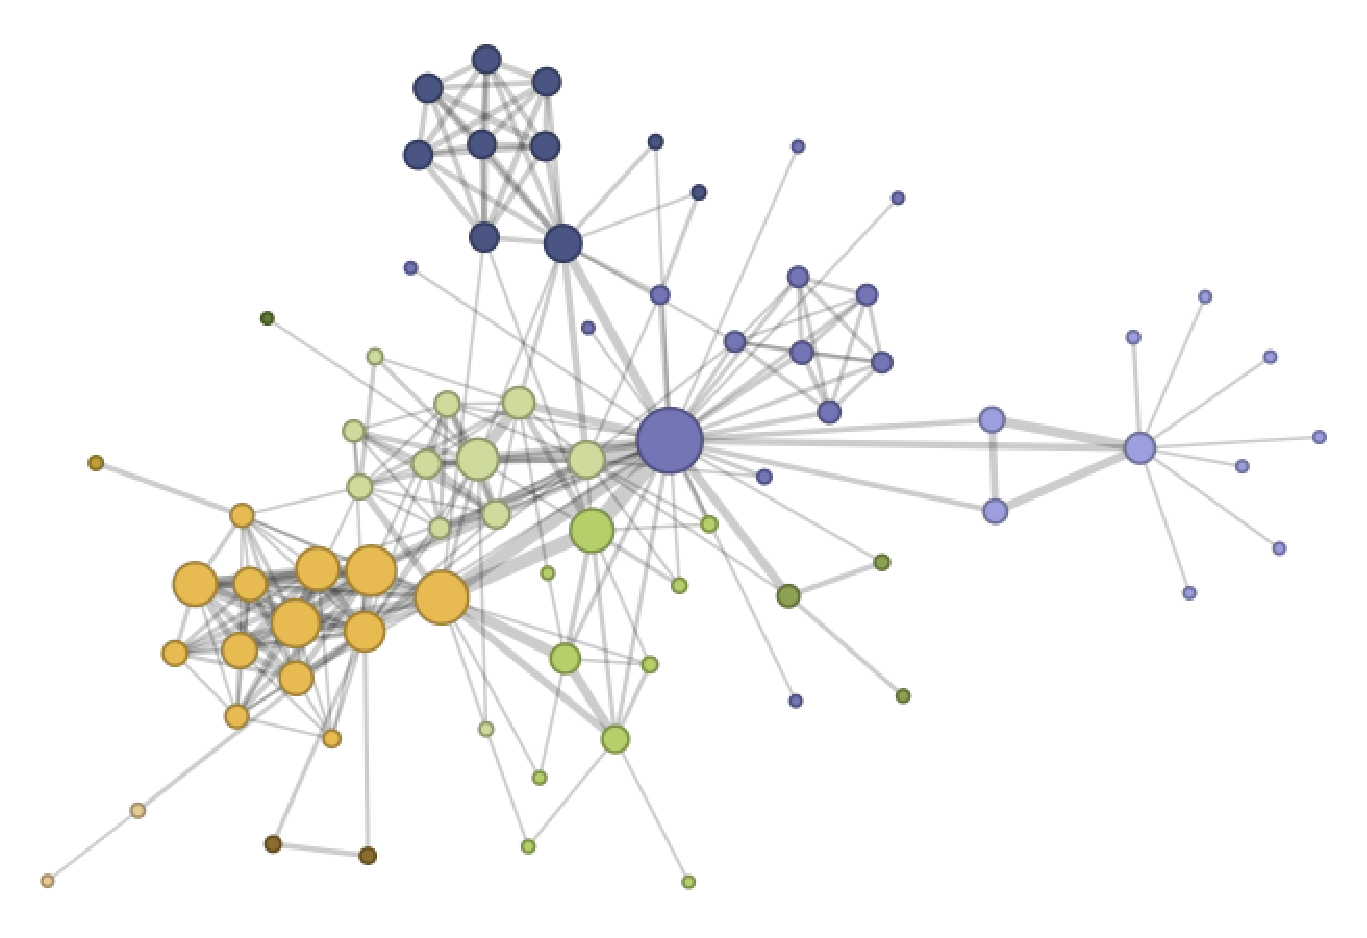
\includegraphics[width=8cm]{figures/force.eps}
	\caption{A force-directed node-link diagram \cite{Knuth:1993:SGP:164984}.}
	\label{fig:forcedirected}
\end{figure}

Networks are often visualized using a force-directed layout, seen in Figure~\ref{fig:forcedirected} \cite{Heer:2010:TTV:1743546.1743567}.  Nodes repel each other, while related nodes become pulled toward each other by links.  The result is an aesthetically pleasing layout where there are relatively few link crossings and links are of approximately similar length.  The color of the node can be used to indicate group membership, while the size can represent the magnitude of some property of the node.  Likewise, the drawing style of the link can be varied to encode different types of relationships. 

\begin{figure}[h]
	\centering
	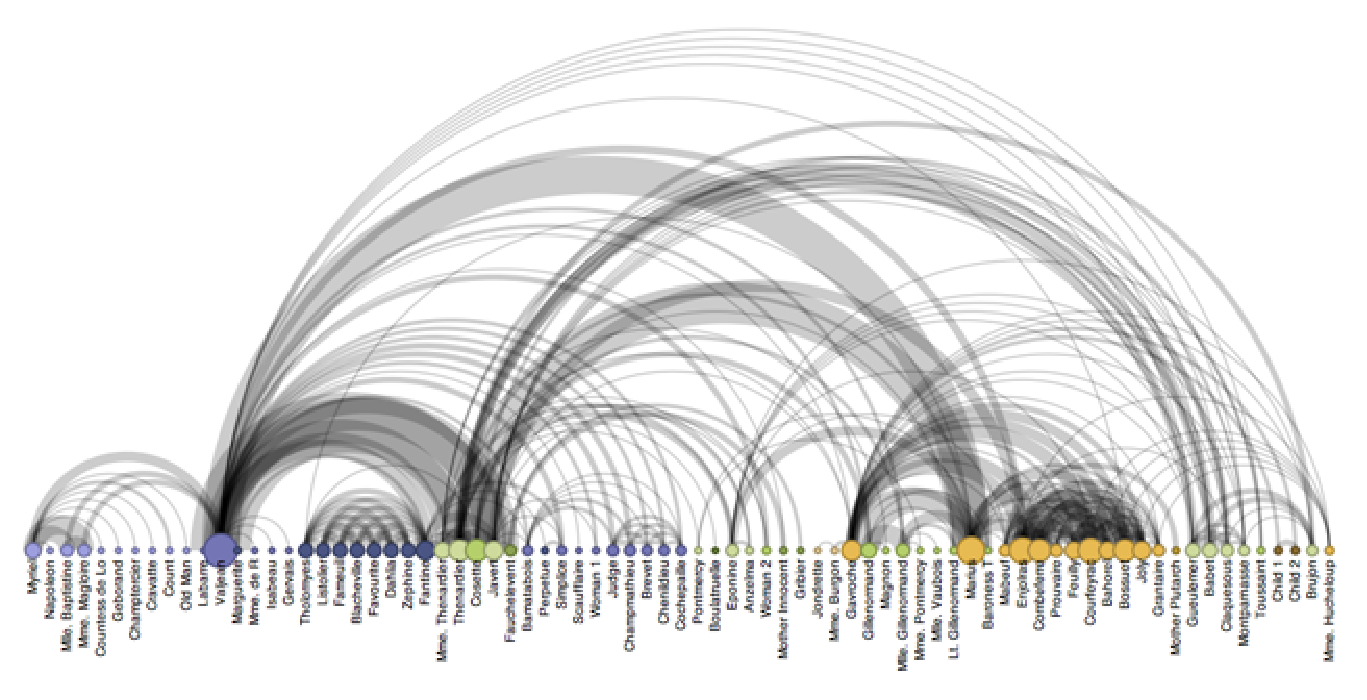
\includegraphics[width=10cm]{figures/arcdiagram.eps}
	\caption{Knuth's arc diagram of \textit{Les Mis\'erables} characters \cite{Knuth:1993:SGP:164984}.}
	\label{fig:arcdiagram}
\end{figure}

An alternative for force-directed layout is an arc diagram.  First coined by Wattenberg \cite{Wattenberg:2002:ADV:857191.857733}, arc diagrams were used by Knuth to illustrate interaction of characters in Victor Hugo's novel \textit{Les} \textit{Mis\'erables}, seen in Figure~\ref{fig:arcdiagram} \cite{Knuth:1993:SGP:164984}.  Each character is represented with a circular node, where size indicates the number of appearances.  The nodes are arranged linearly, colored and ordered according to clusters of characters that appear together frequently.  Semi-transparent arcs are drawn between the characters which appear in the same chapter, with the thickness of the arc representing the number of such appearances.  While the arc diagram may fail to properly depict the structure of a network, Heer et al. point out it is advantageous because the one-dimensionality allows for other features to be easily displayed near the nodes \cite{Heer:2010:TTV:1743546.1743567}.  %Smaller datasets which contain particular clusters of nodes are well suited to arc diagrams. 

\begin{figure}[h]
	\centering
	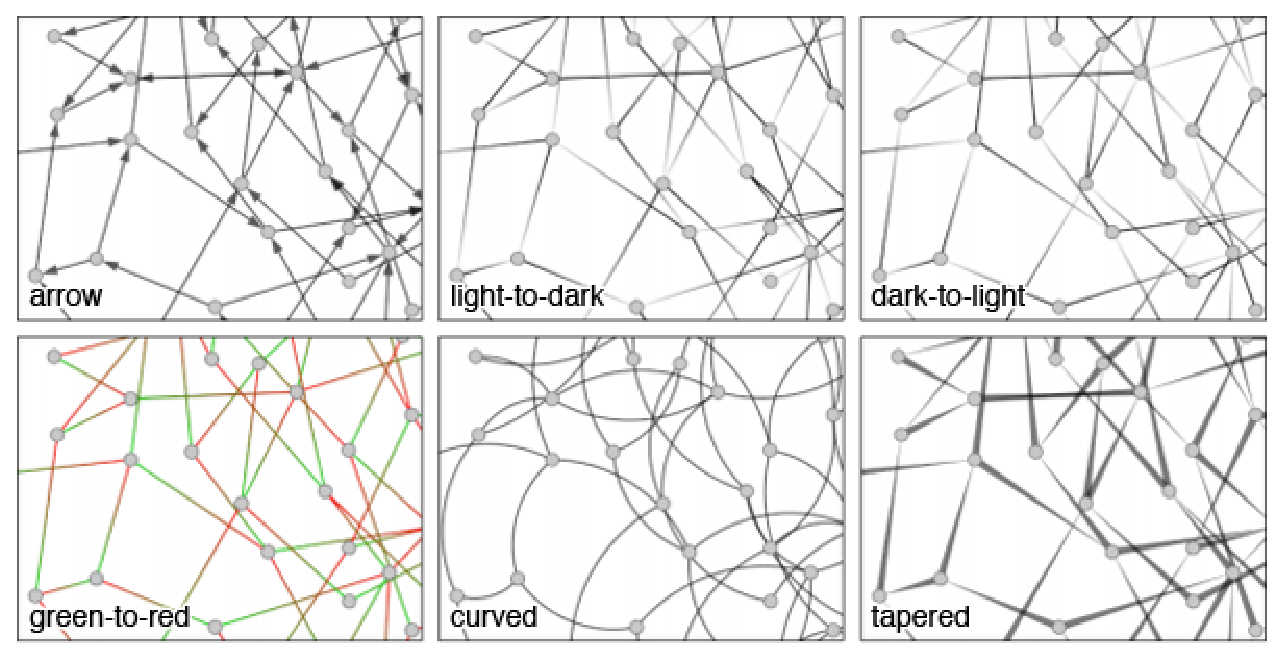
\includegraphics[width=10cm]{figures/directedEdges.eps}
	\caption{Different types of directed edges \cite{Holten:2009:USV:1518701.1519054}.}
	\label{fig:directedEdges}
\end{figure}

Relationships in a network may be directional, such as the predator-prey relationship.  In a visualization of such a network, the direction of the edges must be encoded so these relationships can be understood.  Holten and van Wijk studied the effectiveness of different techniques for indicating directionality of edges in a graph, seen in Figure~\ref{fig:directedEdges} \cite{Holten:2009:USV:1518701.1519054}.  The traditional arrowhead was found to perform poorly, while a tapered edges performed best.  As for an intensity-based direction cue, a dark-to-light representation was found to be clearer than light-to-dark.

\section{Understanding Models}

Models of all kinds---ecological, engineering, statistical, etc.---can benefit from the aid of a visualization.  With even a simple model, patterns and trends may be difficult, if not impossible, to discern from only a table of numerical values.  A simple chart may be all that is necessary to elucidate the mathematics behind a model.  The learning process can be even further enhanced through interaction with the model.  Users can adjust parameter values, perceive a change (or perhaps no change) in the results, and begin to understand the degree of influence different parameters possess.

\begin{figure}[h]
	\centering
	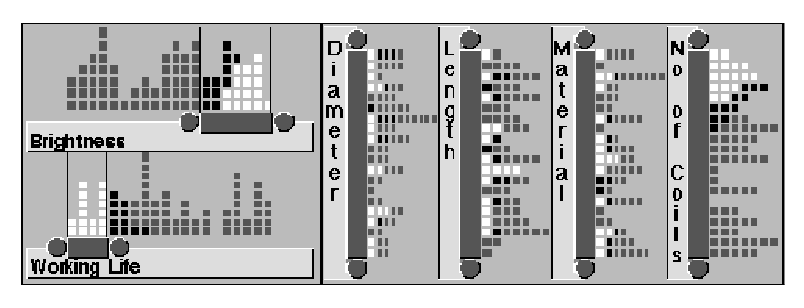
\includegraphics[width=10cm]{figures/influenceExplorer.eps}
	\caption{An example of the Influence Explorer used for the performance of different light bulb designs; white indicates the design passed, black it failed one specification, and grey it failed two specifications \cite{conf/chi/TweedieSDS95}.}
	\label{fig:influenceExplorer}
\end{figure}

A good example of an interaction visualization is the Influence Explorer by Tweedie et al. \cite{conf/chi/TweedieSDS95}.  They developed an interface for understanding the relationships between different attributes in a design process.  Parameter values of the Influence Explorer are initially randomly selected to represent different possible items.  For each attribute, there is a histogram including each of the items.  The attribute ranges are controlled by sliders.  When the user adjusts the slider of a given attribute, all items that are within that range are highlighted on all of the histograms.  Industrial designers found the ability to interactively explore the effects of different parameter ranges to be valuable.
